
% We aim to improve the robustness of BERT~\citep{devlin2018bert} when trained to solve a natural language inference task. Hereafter, we describe the dataset used for this task as well present our methodology.

\subsection{Inference datasets: MNLI and HANS}
\label{sec:dataset}
The MNLI corpus~\citep{williams2017broad} is a popular NLU dataset containing premise/hypothesis pairs annotated with textual entailment information (neutral, entailment or contradiction). Multiple studies have hypothesized that deep learning models tend to capture simple heuristics from the MNLI training data, and do not build an actual understanding of the task. Over the years, a series of diagnostic datasets have been released to test these hypotheses.
The most recent of these datasets, HANS~\citep[Heuristic Analysis for NLI Systems]{linzen2019right}, contains curated templates designed to test the robustness of a model against the following three heuristics for recognizing if a premise entails a hypothesis: lexical overlap (a premise entails any hypothesis built from of a subset of its words), subsequence (a premise entails any of its contiguous subsequences) and constituent (a premise entails all the complete subtrees in its parse tree). In particular, any model relying exclusively on those heuristics would not have a higher than chance classification accuracy on this test set.

\citet{linzen2019right} show that a variety of existing models -- including BERT~\citep{devlin2018bert}, the state-of-the-art model at the time -- perform, overall, worse than chance on classification accuracy of HANS evaluation data. This confirms the hypothesis that models trained on MNLI data tend to learn the three aforementioned heuristics rather than actually understanding the task. To test our methodology, we thus make use of the HANS evaluation dataset, which contains 30,000 examples equally split between the two labels: ``entailment'' and ``non-entailment''.

\subsection{Paraphrase datasets: QQP and PAWS}
\label{sec:dataset_qqp}

The QQP corpus~\citep{qqp} is another widely used NLU dataset containing over 400,000 pairs of sentences annotated as either paraphrase or non-paraphrase. As a consequence of the dataset design, pairs with high lexical overlap have a high probability of being paraphrases. Similarly to MNLI, models trained on QQP are thus prone to learning lexical overlap as a highly informative feature and do not capture the common sense underlying paraphrasing. In order to diagnose this phenomenon, \citet{zhang-etal-2019-paws} propose PAWS (Paraphrase Adversaries from Word Scrambling), a dataset containing over 108,000 sentence pairs well-balanced with respect to the word overlap heuristic. Models with high performance on QQP have been shown to perform terribly on PAWS: for example, the accuracy of BERT is around 91.3\% on QQP and only 32.2\% on PAWS (see Table \ref{tab:paws}).

\subsection{Weak baselines}
% as: here you need to restress that the weak baselines will serve as "bias models", i.e. we hope they will capture biases in the dataset and forgettable example will correspond to those example that do not match the biases (contribution of the paper basically)

We train two models, BoW and BiLSTM, as our weak baselines to compute forgetting statistics of different examples in the training set. We use the term \textit{weak} to emphasize the fact that those models have fewer parameters than the ones we will eventually consider (Section \ref{sec:strong}). Our conjecture is that networks with lower capacity will discover the samples that support the various heuristics described in Sections \ref{sec:dataset} and  \ref{sec:dataset_qqp}. In particular, \emph{forgettable} examples for those models will correspond to sentences that do not verify said heuristics.

Both models are siamese networks, with similar input representations and classification layers.
For the input layer, we lower case and tokenize the inputs into words and initialize their representations with Glove, a 300 dimensional pretrained embedding~\citep{pennington2014glove}.
For the classification task, from the premise and hypothesis vectors $p$ and $h$, we build the concatenated vector $s = [p, h, |p - h|, p \odot h]$ and pass it to a two-layer perceptron classifier. 
To compute $p$ or $h$, the BoW model max-pools the bag of word embeddings,
while the BiLSTM model max-pools the top-layer hidden states of a 2-layer bidirectional LSTM. The hidden size of the LSTMs is set to 200. Overall, BoW contains 560K parameters and BiLSTM 2M.

\begin{table}[t]
\footnotesize
\caption{Number of ``forgettables'' examples (those that are forgotten at least once or never learned) during training along with the accuracy on the MNLI and QQP matched development sets.}
\label{tab:forg_stats}
\centering
\begin{tabular}{llccc}
\toprule
& Model & \# Forg. & \# Balanced Forg. & Acc.\\
\midrule
& BoW         &100,345 & \balancedbow & 64.0\\
\textit{MNLI} & BiLSTM      &76,270 & \balancedlstm  & 69.6\\
& BERT        &32,387 &  \balancedbert & 84.5\\
\midrule
& BoW         &73,478&71,116  & 81.1\\
\textit{QQP} & BiLSTM      &81,754 &76,634   & 84.3 \\
& BERT        &22,372 &20,498   & 91.3 \\
% OLD BALANCED_ALL_FORG:
%\midrule
%& BoW         &73,478&59,477  & 81.1\\
%\textit{QQP} & BiLSTM      &81,754 &68,130   & 84.3 \\
%& BERT        &22,372 &19,014   & 91.3 \\
\bottomrule
\end{tabular}
\end{table}

\subsection{Main models}
\label{sec:strong}
Recently, significant improvements in many NLP tasks have been achieved by deep transformer-based models pretrained on huge amounts of unlabeled data.
Examples of such models include BERT \cite{devlin2018bert}, XLNET \cite{yang2019xlnet}, RoBERTA \cite{roberta2019}, AlBERT \cite{lan2019albert} and SpanBERT \cite{spanBERT2019}.
In this work, we focus on BERT and XLNET, both the base and large versions, and consider them as our strong models. In particular, \bertbase being the model of choice in previous work \cite{clark2019dont,zhang-etal-2019-paws}, it will serve as our default architecture.


% We consider two types of models, BERT and XLNET, both their base and large versions...

\subsection{Computing forgetting events}
\label{sec:forg_stat}
We train our two weak baselines and \bertbase on MNLI and QQP and track the number of times each example is forgotten, following the same procedure described in \citet{toneva2018empirical}. In short, an example is forgotten if it goes from being correctly to incorrectly classified during training (because of gradient updates performed on other examples). 

If an example is forgotten at least once or is never learnt during training, we call it ``forgettable''. %TODO keep forgettable term consistent 
In the following sections, we will consider the forgettable examples for the various models as new fine-tuning sets. In particular, to remove the effect of shifting label distributions, we randomly sample forgettable examples for each label to keep the label distributions of the forgettable sets identical to the ones of MNLI or QQP (i.e., 33\% from each of the three labels in MNLI and 36\% for the paraphrase label in QQP). The results below all make use of the balanced forgettable sets.


\begin{figure}[t]
\centering
  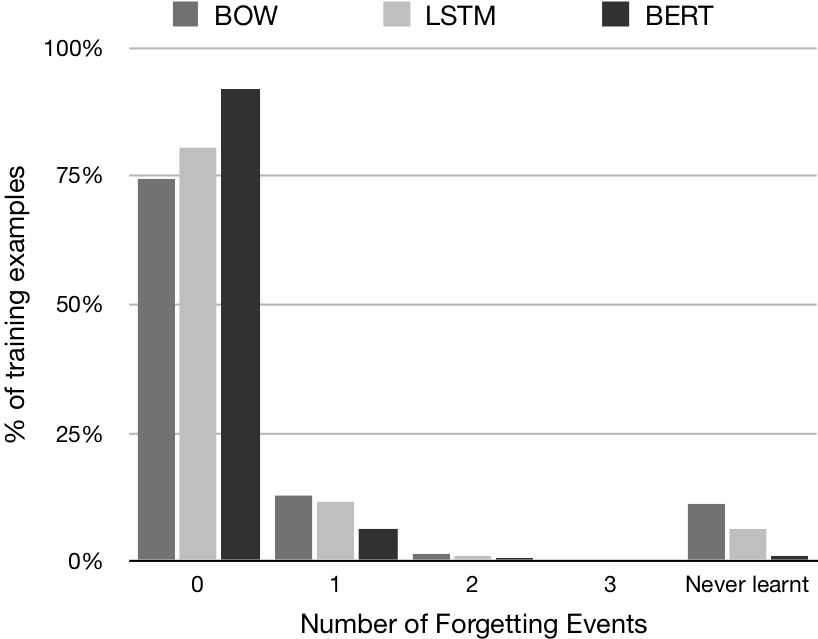
\includegraphics[width=0.45\textwidth]{figures/ex_by_forg.png}
  \caption{Distribution of forgetting events for the three models after five training epochs. As can be seen, a majority of examples are not forgotten during training. We make use of examples 
  with at least one forgetting event in our method for robust NLI models.}
\label{fig:forgcount-freq}
\end{figure}

\iffalse
\begin{figure}[t]
\centering
  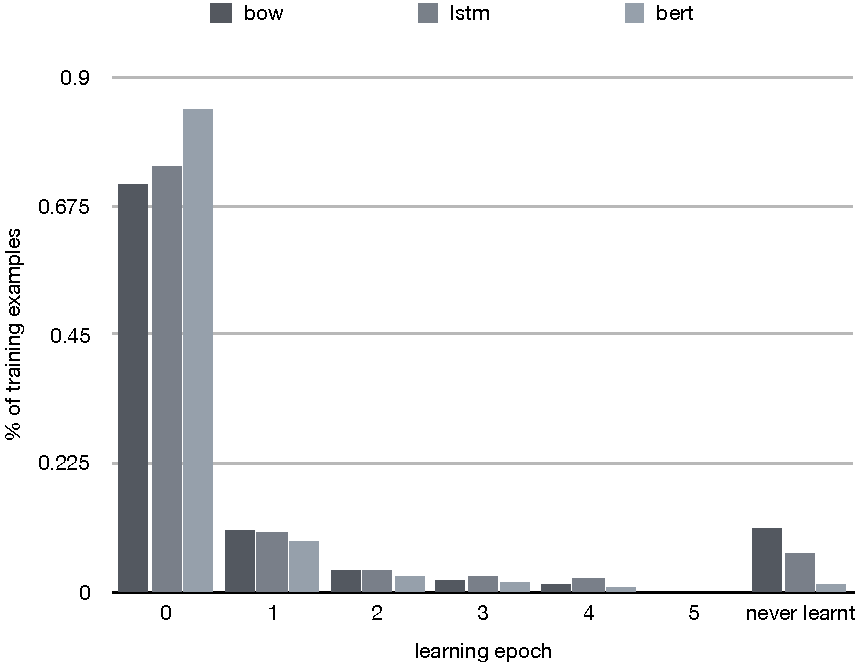
\includegraphics[width=0.45\textwidth]{figures/first_learnt_bar_chart.pdf}
  \caption{Distribution of learning time for training examples during five training epochs. As can be seen, a majority of examples are learnt at the first epoch.}
\label{fig:firstlearnt-freq}
\end{figure}

\begin{figure}[t]
\centering
  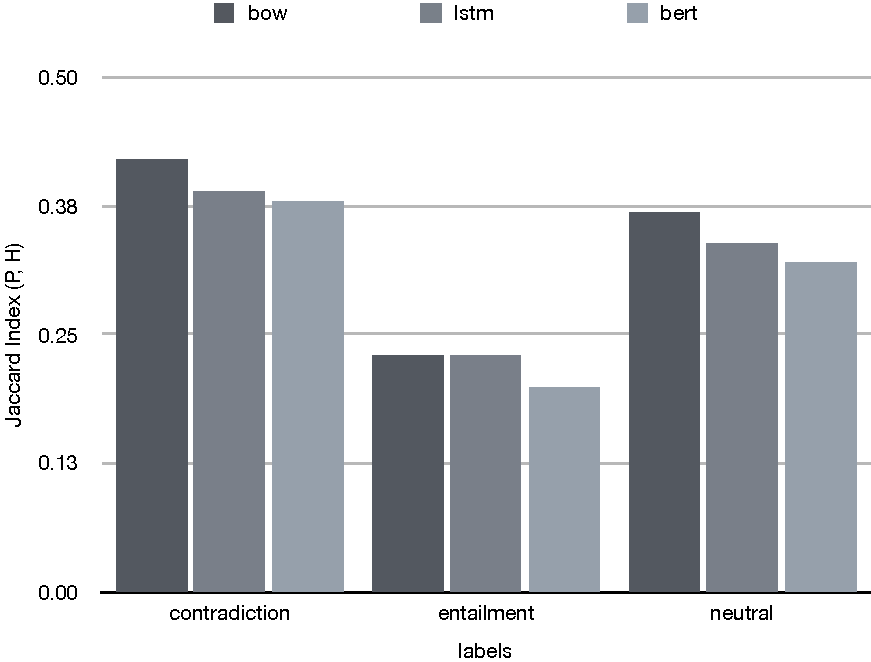
\includegraphics[width=0.45\textwidth]{figures/wordoverlap_unlearned.pdf}
  \caption{Jaccard index between sets of words in Premise and Hypothesis for ``never learned'' examples.}
\label{fig:wordoverlap-unlearned}
\end{figure}

\begin{figure}[t]
\centering
  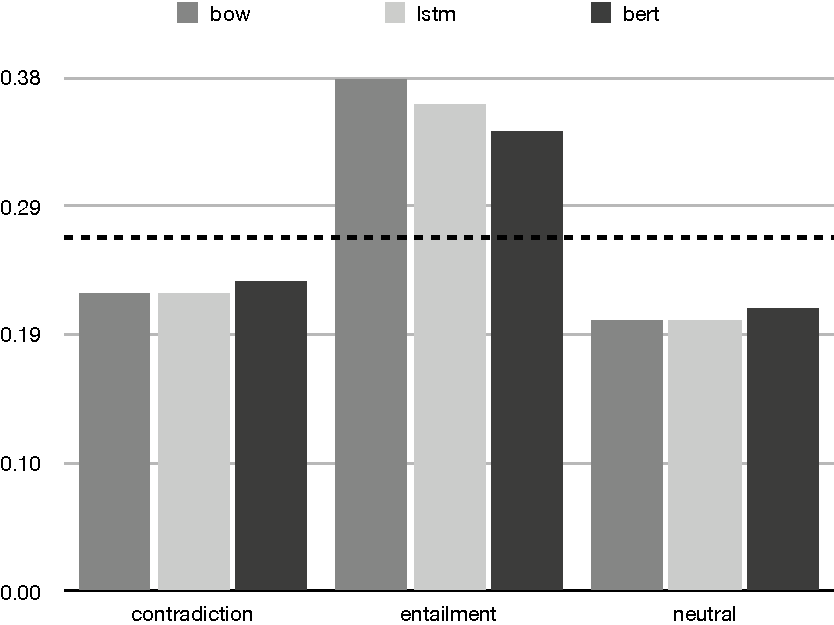
\includegraphics[width=0.45\textwidth]{figures/wordoverlap_unforgettables.pdf}
  \caption{Jaccard index between sets of words in Premise and Hypothesis for ``Unforgettable'' examples.}
\label{fig:wordoverlap-unforg}
\end{figure}

\begin{figure}[t]
\centering
  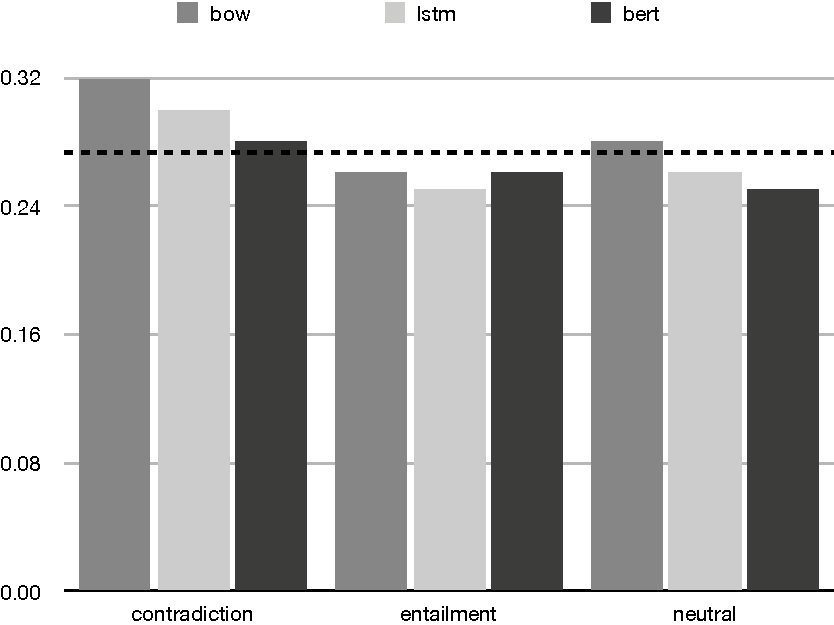
\includegraphics[width=0.45\textwidth]{figures/wordoverlap_forg.pdf}
  \caption{Jaccard index between sets of words in Premise and Hypothesis for ``Forgettable'' examples.}
\label{fig:wordoverlap-forg}
\end{figure}
\fi

\begin{figure}[t]
\centering
  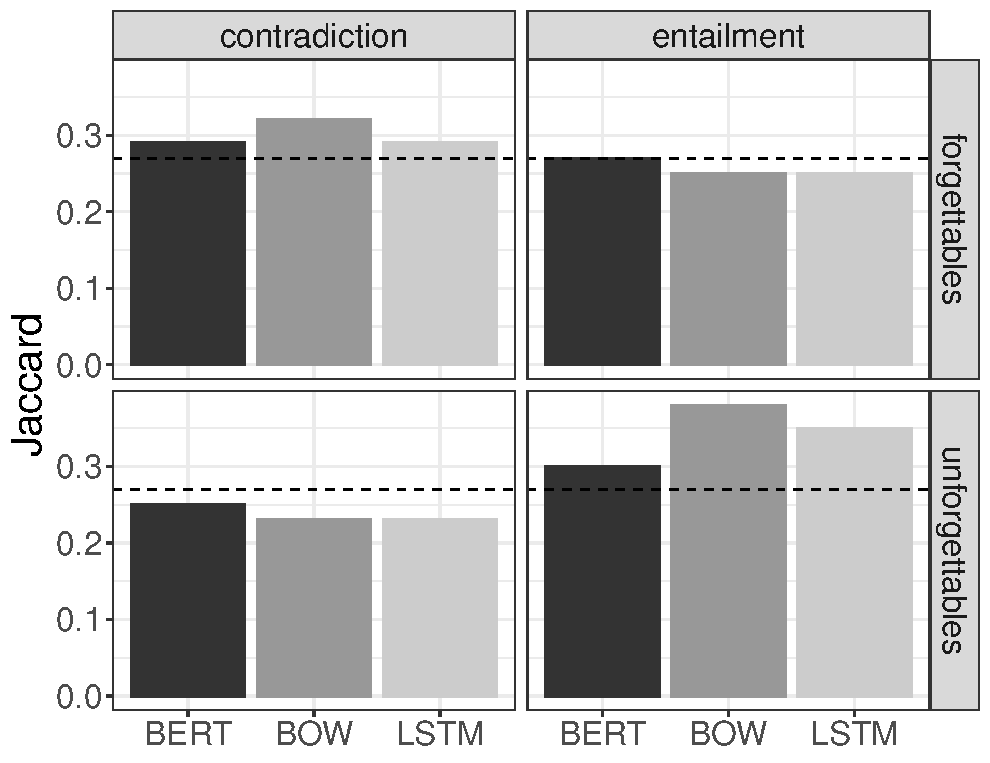
\includegraphics[scale=0.45]{figures/jaccard_plot.pdf}
  \caption{Word overlap between premise and hypothesis as measured by Jaccard similarity in both forgettables and unforgettables examples. For all models, forgettable (unforgettable) examples tend to contain contradiction (entailment) examples with higher than average (dashed line) word overlap which support their usefulness to unlearn the word overlap heuristic.}
\label{fig:wordoverlap-unforg}
\end{figure}

\subsection{Fine-tuning on forgettable examples}
\label{sec:fine_tune}
We adopt a simple strategy to exploit the sets of forgettables computed by the baselines and BERT itself: we first fine-tune our main models on the whole dataset, to get a reasonable prior for the task. We then perform an additional stage of fine-tuning for $3$ epochs on a subset of the training set, composed of the forgettable examples from one of the considered models (i.e. from BoW, BiLSTM or BERT).

\iffalse
\subsection{Comparing our methodology to related work}
\begin{itemize}
    \item The recent work to tackle the brittleness of MNLI trained models all are built based on the prior knowledge about the biases
    in the training dataset. 
    
    
    Notably, \newcite{clark2019dont} introduce a 2 stage process as:
\begin{quote}
        (1)
train a naive model that makes predictions exclusively based on dataset biases, and (2) train
a robust model as part of an ensemble with the
naive one in order to encourage it to focus on
other patterns in the data that are more likely to
generalize
    \end{quote}
    
    \newcite{he2019unlearn} employs a similar approach and uses a bag-of-word, a hypotheis-only and a manually-built bias models, and fits 
    their target model to the residual of these weak baselines.
    
    \newcite{mahabadi2019simple} takes a very similar approach as in \newcite{clark2019dont}.
    
    In compared to these methods, we do not rely on known biases and prior knowledge about the dataset.
    We do however rely on weaker models to compute a more diverse set of forgettables.

\end{itemize}
\fi